
\documentclass{standalone}
\usepackage{fourier}
\usepackage{tikz}
\usetikzlibrary{shapes,shapes.misc,arrows}
\begin{document}
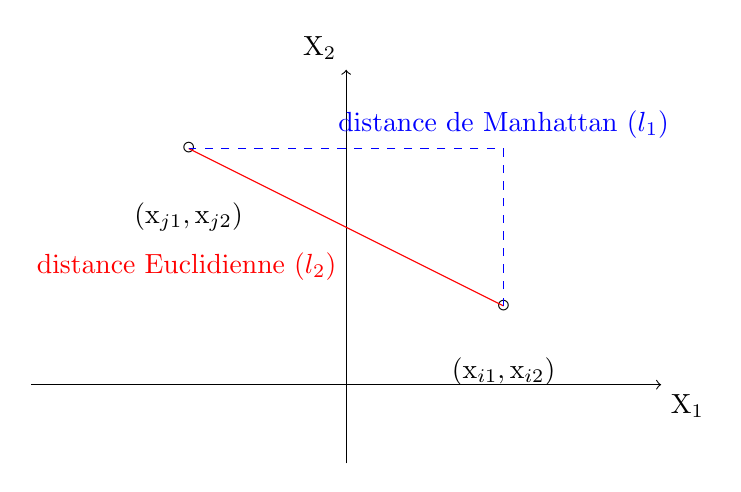
\begin{tikzpicture}
\draw[->] (0, -1) -- (0,4);
\node[above left] at (0,4) {$\mathrm{X}_2$};
\node[below right] at (4,0) {$\mathrm{X}_1$};
\draw[->] (-4, 0) -- (4,0);
\node at (2,1) {$\circ$};
\node at (-2,3) {$\circ$};
\node [below, circle] at (2, 1) {$(\mathrm{x}_{i1}, \mathrm{x}_{i2})$};
\node [below, circle] at (-2, 3) {$(\mathrm{x}_{j1}, \mathrm{x}_{j2})$};
\draw[color=red] (2,1) -- (-2, 3);
\draw[color=blue, dashed] (2,1) -- (2, 3) -- (-2, 3);
\node[above, color = blue] at (2,3) {distance de Manhattan ($l_1$)};
\node[below, left, color=red] at (0,1.5) {distance Euclidienne ($l_2$)};
\end{tikzpicture}

\end{document}
